\documentclass[titlepage, oneside, 14pt]{extbook}

\usepackage{fontspec}
\usepackage[english,bulgarian]{babel}
\usepackage{siunitx}
\usepackage{hyperref}
\usepackage{changepage}
\usepackage[a4paper, margin=1in]{geometry}
\usepackage{titlesec}
\usepackage{setspace}
\usepackage{titling}
\usepackage{parskip}
\usepackage{breqn}
\usepackage{titletoc}
\usepackage{textcomp}
\usepackage{gensymb}
\usepackage{graphicx}
\usepackage[justification=centering]{caption}
\usepackage[backend=biber]{biblatex}

\addbibresource{cites.bib}

\setmainfont{Times New Roman}
\setmonofont{FiraCode Nerd Font}
\renewcommand{\baselinestretch}{1.5}

\renewcommand{\texttt}[1]{{\small\ttfamily #1}}

\makeatletter
\def\verbatim@font{\fontsize{10pt}{12pt}\ttfamily}
\makeatother

\author{Божидар Павлов}
\title{Tetris Display}
\date{2023 г.}

\titleformat{\section}
{\Large\bfseries}
{\thesection.}
{.5em}
{}

\titleformat{\subsection}
{\large\bfseries}
{\thesubsection.}
{.5em}
{}

% \newcommand{\sectionbreak}{\clearpage}
\newcommand{\ard}{Arduino\texttrademark{}}

\setcounter{tocdepth}{1}

\renewcommand{\maketitle}
{
    \begin{titlepage}
        \centering
        {\large\scshape Технологично~училище „Електронни~системи“ към Технически~Университет~–~София\par}
        \vfill
        {\LARGE\scshape\mdseries Курсова работа\par}
        \vspace{1cm}
        {\Huge\bfseries\thetitle\par}
        \vfill
        {\large\bfseries Изготвил \hfill Преподавател\par}
        {\Large\theauthor \hfill Енчо Шахънов\par}
        \vspace{1cm}
        {\large\thedate\par}
    \end{titlepage}
}

\sisetup{locale=FR}

\begin{document}

\maketitle

\setcounter{page}{2}

\section*{Увод}
\addcontentsline{toc}{section}{Увод}

\textit{Tetris Display} е конзола, на която потребителят може да играе
\textit{Тетрис} с приятел. Това е идеалният начин да се забавляват заедно, като се
наслаждават на една от най-популярните игри на всички времена.

\textit{Оригиналната игра} Тетрис е създадена през 1984 г. в Москва от двама компютърни инженери от
\textit{Компютърния център към Руската академия на науките}. В оригиналната игра
единственият играч има за цел да подреди падащи фигури с различна форма,
наречени Тетромино, като изцяло запълнените от фигури редове изчезват.

Този проект представлява модифициран вариант на Тетрис, който се играе от двама играчи,
играещи един срещу друг. Играч 1 подрежда падащите Тетроминота, а Играч 2 управлява кое Тетромино
ще падне на следващия ход. Ако Играч 2 пусне
едно и също парче два пъти последователно, той губи, а пък ако неизчистените редове на Играч 1 достигнат горната част на игралното поле, Играч 2 печели.
\vfill

\begin{figure}[!htbp]
    \centering
    \includegraphics[width=0.6\linewidth]{img/prototype1.png}
    \caption{Първи прототип на \textmd{Tetris Display}}
\end{figure}

\chapter{Теория}

\section{Принцип на работа на проекта}

За реализацията на \textmd{Tetris Display} са необходими микроконтролер,
клавиатура с минимум 5 бутона за контролиране на играта от Играч 1,
ротационен енкодер за избор на следващо Тетромино от Играч 2, екран, изобразяващ текущото
състояние на играта и втори екран, изобразяващ следващото Тетромино.

От момента на пускането си, микроконтролерът започва продължително да чете
текущото състояние на клавиатурата и на ротационния сензор. В случай, че някой
от бутоните за завъртане на падащото Тетромино бъде натиснат от Играч 1, или
ротационният енкодер се завърти от Играч 2, промяната е отразена във вътрешното
състояние на играта.

При натискане на бутона на оста на енкодера от Играч 2, текущата игра бива прекратена и
започва нова игра отначало. Това е реализирано със софтуерно нулиране на UNO платката.

\begin{figure}[!htbp]
    \centering
    \includegraphics[width=0.5\linewidth]{img/functional_diagram.drawio.png}
    \caption{Функционална схема на Tetris Display}
\end{figure}


\section{Избор на хардуерни компоненти за реализацията на проекта}

\subsection{Избор на микроконтролер}

\subsubsection{\textit{\ard{} UNO} ревизия 3}

\textit{\ard{} UNO} \cite{arduino} е най-достъпната, удобна и лесна за програмиране и
употреба платка, както за начинаещи, така и за напреднали, правейки я
най–разпространената \textit{\ard{}} платка. Поради тази причина в интернет има
изключително много информация за това как работи и как трябва да се
програмира. Освен това заедно с платката е предоставена и лесна
и интерактивна среда за програмиране -- \textit{\ard{} IDE}, осигуряваща всичко
необходимо откъм допълнителни библиотеки и софтуер свързани с
програмирането на платката. Тези фактори я правят добър избор за
проекта.

\begin{figure}[!htbp]
    \centering
    \includegraphics[width=0.5\linewidth]{img/arduino.png}
    \caption{Развойна платка \ard{} UNO}
\end{figure}

\textit{UNO} разполага със 14 цифрови входно-изходни порта, 6 от които могат да
са ШИМ\footnote{Широчинно-импулсна модулация} изходи, 6 аналогови входа и
кварцов резонатор на 16 MHz.

В заданието на този курсов проект се изисква задължителната употреба на \ard{} UNO
платка.

\subsection{Избор на клавиатура}

Проектът използва клавиатура с 5 бутона \cite{keypads}, която има аналогов вход за
прочитане на петте състояния на всеки бутон. По този начин се спестява ресурса
на процесора на управляващата платка. Платката на клавиатурата разполага с повече свободни входно/изходни
пинове, които са неизползвани в реализацията на този проект. Платката
разполага и с изходен конектор с три извода. Два от тях са за захранване, третият
е аналогов изход. Клавиатурата е подходяща за връзка както с развойните платки
UNO, NANO, така и PIC, MSP и други.

\begin{figure}[!htbp]
    \centering
    \includegraphics[width=0.5\linewidth]{img/keypad.png}
    \caption{Аналогова клавиатура}
\end{figure}

Схемата на свързване на тази клавиатура, изобразена на фигура \ref{keypad_circuit} се състои от 5 ключа, които, ако са затворени,
дават успоредно свързаните резистори на късо, променяйки изходното напрежение. То може
да бъде четено тривиално от аналогов пин на развойната платка UNO.

\begin{figure}[!htbp]
    \centering
    \includegraphics[width=0.5\linewidth]{img/keypad_circuit.png}
    \caption{Принципна схема на аналогова клавиатура}
    \label{keypad_circuit}
\end{figure}

\subsection{Избор на сензор за завъртане}

\subsubsection{Потенциометър}

За входно устройство възможен избор би бил потенциометър \cite{potent} --
резистор с 3 извода, с който е възможно при промяна на съпротивлението му
чрез плъзгащ контакт в електрическата верига да се променя изходното напрежение.

\begin{figure}[!htbp]
    \centering
    \includegraphics[width=0.3\linewidth]{img/potentiometer.png}
    \caption{Кръгъл потенциометър}
\end{figure}

На фигура \ref{potentiometer_circuit} е изобразена еквивалентната електрическа схема на един потенциометър.
Ако свържем високия потенциал от входа към захранващия пин на нашия микроконтролер,
а високия -- към някой от заземените (GND) пинове, то тогава потенциалната разлика между
средната точка и нулата може да бъде управлявана от ориентацията на плъзгача.

\begin{figure}[!htbp]
    \centering
    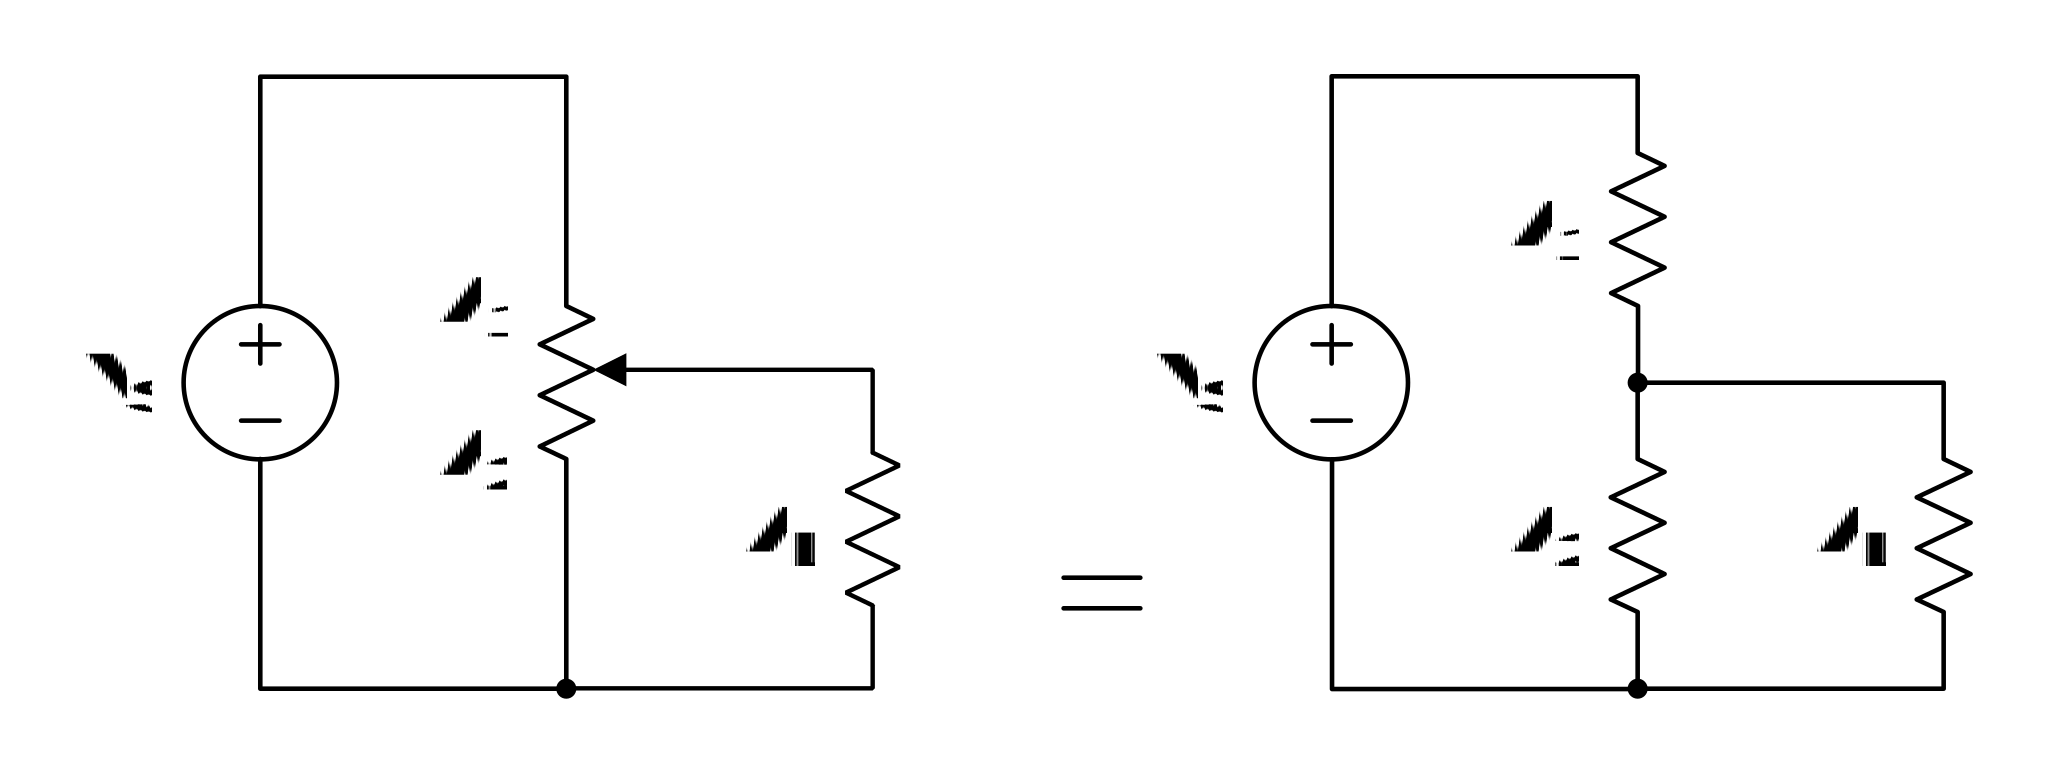
\includegraphics[width=0.7\linewidth]{img/potentiometer_circuit.png}
    \caption{Потенциометър в електрическа верига и неговата еквивалентна схема}
    \label{potentiometer_circuit}
\end{figure}


Ако свържем третия извод на потенциометъра към някой от аналоговите входове на UNO микроконтролера,
ние ще можем софтуерно да четем уникална числова стойност от 0 до 1023, описваща настоящата позиция
на плъзгача. Тази стойност може да управлява изборът на тетромино в нашата игра.

Главният недостатък на потенциометъра за проекта е, че плъзгачът може да бъде завъртан
единствено в интервал от $\frac{3}{4}$ от целия кръг, но за реализацията на този проект е необходимо
той да може свободно да бъде завъртан двупосочно в целия интервал от
360\textdegree{}. Потенциометърът е полезен в случаи, в които искаме да научим точната настояща позиция
на плъзгача, но за управлението тя не е важна, тъй като промяната на изборът на Тетромино се управлява
от промяната на ориентацията и посоката на въртене.

\subsubsection{Ротационен енкодер}

Следващият избор за сензор за въртене е ротационен енкодер \cite{encodertut}. Подобно на потенциометъра, ротационният енкодер представлява
електромеханично устройство, което преобразува ъгловото положение или движението на вал или ос
в аналогови или цифрови изходни сигнали, но за разлика от него, той може да
бъде завъртан в интервал от 360\textdegree{} -- както в посока на часовниковата
стрелка, така и в обратна на нея.

\begin{figure}[!htbp]
    \centering
    \includegraphics[width=0.5\linewidth]{img/encoder.png}
    \caption{Модул ротационен енкодер}
\end{figure}

Съществуват два основни типа ротационни енкодери: абсолютни и инкрементални. Изходът на абсолютния енкодер показва текущото
положение на вала, което го прави преобразовател на ъгъл. Изходът на
инкременталния енкодер предоставя информация за движението на вала, която
обикновено се обработва на друго място в информация като позиция, скорост и
разстояние.

\subsubsection*{Краен избор}

Тъй като на нас ни е необходимо да знаем по какъв начин е придвижен валът, за
реализацията на този проект е използван инкрементален цифров ротационен
енкодер.

\subsection{Избор на дисплеи}

Проектът използва два матрични \ref{matrix} LED дисплея -- един с резолюция 32x8 пиксела и един с резолюция 8x8 пиксела.
Дисплей 1 се управлява от четири MAX7219 \cite{displaytut} драйвера за дисплеи, всеки от които управлява зона
от 8x8 пиксела. Драйверите са свъзрани последователно, като част от FC-16
модула. Микроконтролерът управлява състоянието на дисплея чрез серийна комуникация,
използваща SPI протокола. Дисплей 2 е управляван от единичен MAX7219 модул (фиг. \ref{genericmod}).

\begin{figure}[!htbp]
    \centering
    \includegraphics[width=0.5\linewidth]{img/display_matrix.jpg}
    \caption{LED матрица с размер 8x8 без модул за управление}
    \label{matrix}
\end{figure}

\begin{figure}[!htbp]
    \centering
    \includegraphics[width=0.5\linewidth]{img/display.png}
    \caption{MAX7219 FC-16 LED матрица с размер 32x8}
\end{figure}

\begin{figure}[!htbp]
    \centering
    \includegraphics[width=0.5\linewidth]{img/display_generic.png}
    \caption{MAX7219 LED матрица с размер 8x8}
    \label{genericmod}
\end{figure}


\chapter{Практика}

\section{Изходен код}

Тъй като реализацията на играта Тетрис изисква нетривиално количество изходен код,
в тази документация са прикачени единствено ключовите части. Целият код може да
бъде намерен в GitHub хранилището на проекта \cite{github}.

\subsection{Кодиране на падащото Тетромино}

В Тетрис съществуват седем различни Тетроминота, като всяко едно от тях може да бъде обърнато по 4 начина и
всяко от тях може да бъде нанесено върху мрежа с размер 4x4 по начина, изобразен на фигура \ref{tetrogrid}.

\begin{figure}[!htbp]
    \centering
    \includegraphics[width=0.5\linewidth]{img/tetrominoes_grid.drawio.png}
    \caption{\textit{Тетроминота}, нанесени върху 4x4 мрежа с координатна система}
    \label{tetrogrid}
\end{figure}

\newpage

Съответно в код се представят празните и запълнените позиции на фигурите като масив от символни низове.

\begin{verbatim}
constexpr char *tetrominoes[] =
{
  "..X."
  "..X."
  "..X."
  "..X.",

  "..X."
  ".XX."
  "..X."
  "....",

  // ...

  "..X."
  "..X."
  ".XX."
  "....",
};
constexpr size_t num_tetrominoes =
  sizeof tetrominoes / sizeof *tetrominoes;
\end{verbatim}

\begin{sloppypar}Вида Тетромино се представя с индекс от този масив -- число от 0 до \texttt{num_tetrominoes}.\end{sloppypar}

Различните ориентации на всяко едно Тетромино се получават като индексираме символните низове в различен ред.
Всеки квадрат от 4x4 мрежата представлява точка от координатна система, описана на фирура \ref{tetrogrid}.
Нека точките в тази система имат координати \texttt{dx} и \texttt{dy}. Всичките възможни видове индексиране са описани по следния начин:

\begin{figure}[!htbp]
    \centering
    \includegraphics[width=0.6\linewidth]{img/tetromino_rotations.drawio.png}
    \caption{Формули за индексиране на символните низове на Тетроминотата}
\end{figure}

\begin{verbatim}
const char (*rotations[])(int dx, int dy, int tetromino_idx) =
{
  [tetrominoes](int dx, int dy, int tetromino_idx)
    { return tetrominoes[tetromino_idx][dy * 4 + dx]; },
  [tetrominoes](int dx, int dy, int tetromino_idx)
    { return tetrominoes[tetromino_idx][12 + dy - (dx * 4)]; },
  [tetrominoes](int dx, int dy, int tetromino_idx)
    { return tetrominoes[tetromino_idx][15 - (dy * 4) - dx]; },
  [tetrominoes](int dx, int dy, int tetromino_idx)
    { return tetrominoes[tetromino_idx][3 - dy + (dx * 4)]; },
};
constexpr size_t num_rotations = sizeof rotations / sizeof *rotations;
\end{verbatim}

За оптимизация на бързодействието на алгоритъма, всяка ориентация представлява C++ ламбда функция, взимаща
координатите \texttt{dx} и \texttt{dy} и индекса на вида Тетромино и връща \texttt{'.'}, ако тази позиция е празна
и \texttt{'X'}, ако тя е запълнена.

Указатели към функциите се пазят в масива \texttt{rotations}, който е с дължина \texttt{num_rotations}. Следователно
ориентацията на едно Тетромино се представя като индекс в този масив.

Освен вида и ориентацията на едно Тетромино, в цифровото представяне на едно Тетромино се съхраняват и неговите
координати \texttt{x} и \texttt{y}, спрямо горния ляв пиксел на дисплея.

Така изглежда структурата за едно Тетромино:

\begin{verbatim}
struct Tetromino
{
  int x, y, type, rotation;
} tetromino;
\end{verbatim}

\texttt{tetromino} е глобална променлива за падащата фигура в играта.

За тази структура съществуват следните методи:

\begin{itemize}
  \item \texttt{Tetromino::move_left()} и \texttt{Tetromino::move_right} -- премества позицията с 1 наляво/надясно
  \item \texttt{Tetromino::rotate()} -- завърта на 90\textdegree{}
  \item \texttt{Tetromino::apply_gravity()} -- премества позицията с 1 надолу
  \item \texttt{Tetromino::place()} -- утвърждава окончателно настоящата
    позиция, като я прибавя към вече поставените парчета (т. \ref{stack}) и нулира позицията на Тетроминото.
  \item \texttt{Tetromino::drop()} -- премества позицията надолу, докато не стигне до най-ниското, достижимо ниво
\end{itemize}

\subsection{Кодиране на поставените парчета}
\label{stack}

Поставените парчета се съхраняват в двумерен масив от тип \texttt{bool} с размери 8x32:

\begin{verbatim}
bool stack[DPY_WIDTH][DPY_HEIGHT]{false};
\end{verbatim}

Ако \texttt{stack[x][y] == true}, позицията на дисплея с координати \texttt{x}, \texttt{y} е запълнена.

\subsection{Четене на натиснат клавиш от клавиатурата}

С цел по-четим код, се дефинира изброим тип, изреждащ всичките клавиши.

\begin{verbatim}
enum struct Key : byte
{
  None, Up, Down, Left, Right, Drop
};
\end{verbatim}

Функцията \texttt{get_pressed_key()} връща стойност от \texttt{Key} изброимия
тип, описваща натиснатия клавиш в момента на нейното извикване.

Стойностите на напрежението на аналоговия сигнал са нестабилни и поради тази причина е необходимо
да се прави проверка в интервал около желаната стойност.

\begin{verbatim}
#define APPROX_EQ(val, ref) ((ref)-50 <= (val) && (val) <= (ref)+50)

Key key = Key::None;

Key get_pressed_key(uint8_t pin)
{
  int val = analogRead(pin);
  Key old_key = key;
  if (APPROX_EQ(val, 144))
    key = Key::Up;
  else if (APPROX_EQ(val, 328))
    key = Key::Down;
  else if (APPROX_EQ(val, 0))
    key = Key::Left;
  else if (APPROX_EQ(val, 504))
    key = Key::Right;
  else if (APPROX_EQ(val, 738))
    key = Key::Drop;
  else
    key = Key::None;
  return key != old_key ? key : Key::None;
}
\end{verbatim}

\subsection{Прочитане на състоянието на ротационния енкодер}

За по-четим код, се дефинира структура, съдържаща необходимите методи.

\begin{verbatim}
struct Encoder
{
  uint8_t clk_pin, dt_pin, sw_pin;
  int rotation=0, last_clk=0;
  bool is_clockwise=false, button=false, has_rotated=false,
    was_button_pressed=false;

  Encoder(uint8_t clk_pin, uint8_t dt_pin, uint8_t sw_pin)
    : clk_pin(clk_pin), dt_pin(dt_pin), sw_pin(sw_pin)
  {
  }

  void begin();
  void read();
};

\end{verbatim}
Като полета се запазват номерата на цифровите пинове, към които са свързани изходите на енкодера:

\begin{itemize}
    \item CLK
    \item DT
    \item SW
\end{itemize}

Тяхната функция е документирана на по-късен етап. % КЪДЕ

Структурата също така съхранява полета за настоящото състояние на енкодера.


\subsubsection{Инициализация на енкодера}

\texttt{Encoder::begin()} функцията инициализира необходимите цифрови пинове като
входни за микроконтролера и запазва настоящото състояние на CLK пина.

\begin{verbatim}
void Encoder::begin()
{
  pinMode(clk_pin, INPUT);
  pinMode(dt_pin, INPUT);
  pinMode(sw_pin, INPUT_PULLUP);
  last_clk = digitalRead(clk_pin); 
}
\end{verbatim}

\begin{verbatim}
constexpr int ENC_CLK_PIN=2, ENC_DT_PIN=3, ENC_SW_PIN=4;

Encoder enc(ENC_CLK_PIN, ENC_DT_PIN, ENC_SW_PIN);

void setup()
{
  enc.begin();
  // ...
}
\end{verbatim}

\subsubsection{Прочитане на състоянието на енкодера}

\texttt{Encoder::read()} функцията прочита състоянието от цифровите пинове, използвани от енкодера, в полетата на структурата.

Ако стойността на CLK е променена спрямо предходното му състояние, енкодерът е бил завъртян, като можем да научим
посоката от DT пина.

От SW изхода на енкодера разбираме дали бутонът е натиснат.

\begin{verbatim}
void Encoder::read()
{
  int current_clk = digitalRead(clk_pin);
  if (!last_clk && current_clk)
  {
    if (digitalRead(dt_pin))
      ++rotation, is_clockwise=true;
    else
      --rotation, is_clockwise=false;
    has_rotated = true;
  }
  else
    has_rotated = false;
  last_clk = current_clk;

  bool new_button = !digitalRead(sw_pin);
  was_button_pressed = !button && new_button;
  button = new_button;
}
\end{verbatim}

\subsection{SPI комуникация с матричния дисплей}

За SPI комуникация с дисплеите е използвана \texttt{MD_MAX72xx} библиотеката от \textit{majicDesigns} \cite{library}.

По следният начин се дефинира и инициалзира дисплеите:

\begin{verbatim}
constexpr int DPY_WIDTH=8, DPY_HEIGHT=32;
constexpr int DPY_CS_PIN=10;

MD_MAX72XX dpy(MD_MAX72XX::FC16_HW, DPY_CS_PIN, DPY_HEIGHT/8);

void setup()
{
  // ...
  dpy.begin();
}
\end{verbatim}

\subsubsection{Обновяване на изображението на 32x8 дисплея}

След всяка съществена промяна на състоянието на играта е необходимо изображението на дисплея да бъде обновено.
Това става с \texttt{redraw()} функцията, която е извиквана при необходимост.

\begin{verbatim}
void redraw()
{
  dpy.clear();                // Целият дисплей се нулира.
  draw_tetromino(tetromino);  // Падащото Тетромино се изобразява.
  draw_stack();               // Поставените Тетроминота се изобразяват.
}
\end{verbatim}

Рисуването на Тетромино се изпълнява по следния начин:

\begin{verbatim}
void draw_tetromino(Tetromino t)
{
  for (int dx=0; dx<4; ++dx)
    for (int dy=0; dy<4; ++dy)
      dpy.setPoint(DPY_WIDTH-t.x-1-dx, DPY_HEIGHT-t.y-1-dy,
          rotations[t.rotation](dx, dy, t.type) == 'X');
}
\end{verbatim}

Тъй като координатната система, използвана от кода, и координатната система на 32x8 MAX7219 дисплея не съвпадат,
е необходимо да се извърши трансформация на коодринатите. По подобен начин се рисуват и вече поставените парчета:

\begin{verbatim}
void draw_stack()
{
  for (int x=0; x<DPY_WIDTH; ++x)
    for (int y=0; y<DPY_HEIGHT; ++y)
      if (stack[x][y])
        dpy.setPoint(DPY_WIDTH-x-1, DPY_HEIGHT-y-1, true);
}
\end{verbatim}

\section{Свързване на електронните компоненти\label{wiring}}

При свързването на електронните компоненти, захранването (+5V) и земята (GND) е
необходимо да бъдат общи за всичките компоненти. Допълнително, информационните
и синхронизиращите входове на SPI комуникацията с двата дисплея се изисква да са
свързани с обща шина. За реализирането на това, този проект си служи с breadboard. \cite{breadboard}

\begin{figure}[!htbp]
    \centering
    \includegraphics[width=0.5\linewidth]{img/breadboard.png}
    \caption{Breadboard}
\end{figure}

\subsection{Свързване на MAX7219 дисплеите}

Пиновете на 32x8 дисплея се свързват със следните пинове на \ard{} UNO микроконтролера:

\begin{center}
  \begin{tabular}{c|c}
    Пин от MAX7219 & Пин от \ard{} UNO \\ 
    \hline
    VCC & +5V \\  
    GND & GND \\  
    DIN & Цифров 11 \\  
    CS & Цифров 10 \\  
    CLK & Цифров 13
  \end{tabular}
\end{center}

\begin{figure}[!htbp]
    \centering
    \includegraphics[width=0.5\linewidth]{img/display_wiring.png}
    \caption{Свързване на MAX7219 FC-16 модул}
\end{figure}

Пиновете на 8x8 дисплея се свързват със следните пинове на \ard{} UNO микроконтролера:

\begin{center}
  \begin{tabular}{c|c}
    Пин от MAX7219 & Пин от \ard{} UNO \\ 
    \hline
    VCC & +5V \\  
    GND & GND \\  
    DIN & Цифров 11 \\  
    CS & Цифров 8 \\  
    CLK & Цифров 13
  \end{tabular}
\end{center}

\subsection{Свързване на аналоговата клавиатура}

Пиновете на аналоговата клавиатура се свързват със следните пинове на \ard{} UNO микроконтролера:

\begin{center}
  \begin{tabular}{c|c}
    Пин от клавиатура & Пин от \ard{} UNO \\ 
    \hline
    OUT & Аналогов 0 \\  
    VCC & +5V \\  
    GND & GND
  \end{tabular}
\end{center}

\subsection{Свързване на ротационния енкодер}

Пиновете на ротационния енкодер се свързват със следните пинове на \ard{} UNO микроконтролера:

\begin{center}
  \begin{tabular}{c|c}
    Пин от енкодера & Пин от \ard{} UNO \\ 
    \hline
    CLK & Цифров 2 \\  
    DT & Цифров 3 \\  
    SW & Цифров 4 \\
    + & +5V \\
    GND & GND
  \end{tabular}
\end{center}

\vspace{2cm}

\begin{figure}[!htbp]
    \centering
    \includegraphics[width=0.5\linewidth]{img/encoder_wiring.png}
    \caption{Свързване на ротационен енкодер}
\end{figure}

\section{Захранване на \ard{} UNO}

Проектът се захранва чрез главния \ard{} UNO микроконтролер, като това може да стане по три начина:

\begin{itemize}
  \item Чрез USB-B кабел захванващ кабел
  \item Чрез Power Jack захранващ кабел 
  \item Чрез 9V батерия, чиито полюси са свързани чрез конектор съответно към $V_in$ и GND пинове на микроконтролера.
\end{itemize}

%\begin{figure}[!htbp]
%    \centering
%    \includegraphics[width=0.6\linewidth]{img/power_jack.png}
%    \caption{Power Jack}
%\end{figure}

\section{Програмиране на \ard{} UNO}

Процесът на програмиране на микроконтролера включва следните стъпки:

\begin{enumerate}
  \item Свързване на електронните компоненти (т. \ref{wiring})
  \item Свързване на \ard{} UNO микроконтролера към компютър с USB-B кабел.
  \item Изтегляне на инсталационен скрипт за Tetris Display от GitHub \cite{github} на компютъра.
  \item Изпълняване на инсталационния скрипт от компютъра.
\end{enumerate}

\subsubsection{Изтегляне на инсталационен скрипт за Tetris Display от GitHub на компютъра.}

Всичките издания на Tetris Display са видими в Releases секцията от GitHub хранилището на проекта \cite{github}.
За различните операционни системи е необходимо да се използва различен инсталационен скрипт:

\subsubsection{Изпълняване на инсталационния скрипт от компютъра.}

\begin{center}
  \begin{tabular}{c|c}
    Операционна система & Име на файл \\ 
    \hline
    GNU/Linux & \texttt{tetris_display_install_gnu.sh} \\  
    Windows & \texttt{tetris_display_install_win.ps1} \\  
  \end{tabular}
\end{center}

Необходимо е скриптът за операционната система на компютъра да бъде изтеглен от GitHub хранилището,
да бъде изпълнен и да бъдат следвани указанията, написани в конзолния прозорец.

След успешно изпълнение, скриптът ще завърши със следното съобщение:

\begin{verbatim}
...
Tetris Display successfully flashed!
\end{verbatim}

В този случай \ard{} UNO микроконтролерът е успешно програмиран и играта ще бъде пусната на свързания дисплей.

\chapter*{Заключение}
\addtocontents{toc}{\bigskip}
\addcontentsline{toc}{section}{Заключение}

В заключение, проектът Tetris Display представя нова вариация на старата и харесвана игра Тетрис,
която е играна от двама играчи.

В бъдеще Tetris Display може да бъде развит с въвеждането на цветен дисплей, фонова музика и звукови ефекти
по време на играта, помагащи на играчите да се потопят в нея.

\textmd{Tetris Display} е идеална конзола за партита, рождени дни или просто за една релаксираща
игра с приятели.

\printbibliography[heading=bibliography,title={Използвана литература}]
\addcontentsline{toc}{section}{Използвана литература}

\tableofcontents

\addcontentsline{toc}{section}{Съдържание}

\end{document}
